% Created 2019-10-10 jue 11:43
\documentclass[presentation,aspectratio=169]{beamer}
\usepackage[utf8]{inputenc}
\usepackage[T1]{fontenc}
\usepackage{fixltx2e}
\usepackage{graphicx}
\usepackage{longtable}
\usepackage{float}
\usepackage{wrapfig}
\usepackage{rotating}
\usepackage[normalem]{ulem}
\usepackage{amsmath}
\usepackage{textcomp}
\usepackage{marvosym}
\usepackage{wasysym}
\usepackage{amssymb}
\usepackage{hyperref}
\tolerance=1000
\usepackage{khpreamble}
\usepackage{amssymb}
\DeclareMathOperator{\shift}{q}
\DeclareMathOperator{\diff}{p}
\usetheme{default}
\author{Kjartan Halvorsen}
\date{\today}
\title{Computerized Control - Polynomial pole placement (RST)}
\hypersetup{
  pdfkeywords={},
  pdfsubject={},
  pdfcreator={Emacs 25.3.50.2 (Org mode 8.2.10)}}
\begin{document}

\maketitle


\section{Intro}
\label{sec-1}

\begin{frame}[label=sec-1-1]{Goal of today's lecture}
\begin{itemize}
\item Understand how to design an RST controller
\end{itemize}
\end{frame}

\section{2-dof controller}
\label{sec-2}

\begin{frame}[label=sec-2-1]{Two-degree-of-freedom controller}
\begin{center}
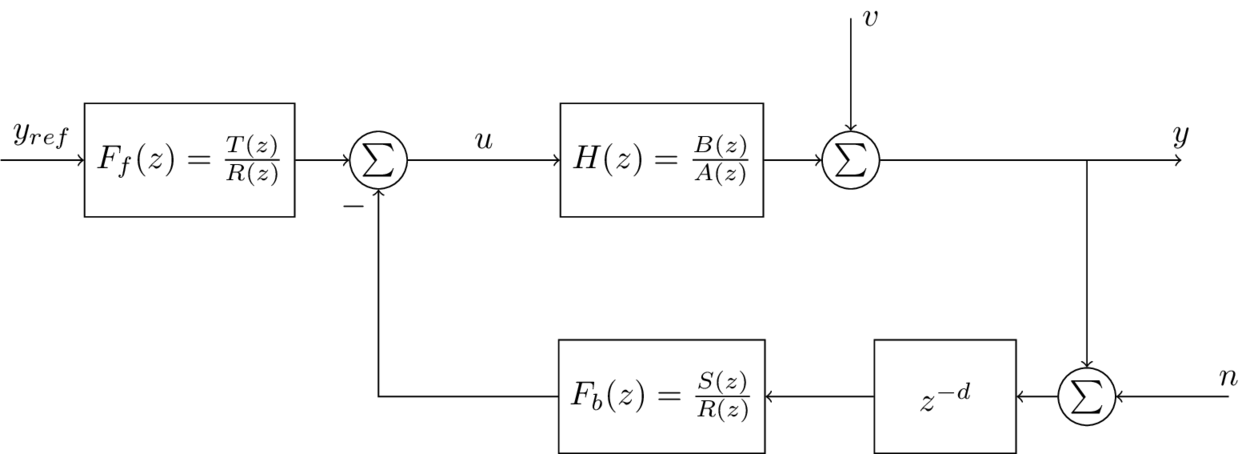
\includegraphics[width=0.8\linewidth]{../../figures/2dof-block-explicit}
\end{center}
\end{frame}

\section{RST}
\label{sec-3}

\begin{frame}[label=sec-3-1]{Procedure}
Given plant model \(H(z)=\frac{B(z)}{A(z)}\) and specifications on the desired closed-loop poles \(A_{cl}(z)\)
\begin{enumerate}
\item Find polynomials \(R(z)\) and \(S(z)\) with \(n_R \ge n_S\) such that 
\[ A(z)R(z)z^{d} + B(z)S(z) = A_{cl}(z) \]
\item Factor the closed-loop polynomials as \(A_{cl}(z) = A_c(z)A_o(z)\), where \(n_{A_o} \le n_R\). Choose
\[T(z) = t_0 A_o(z),\] where \(t_0 = \frac{A_c(1)}{B(1)}\).
\end{enumerate}

The control law is then
\[ R(q) u(k) = T(q)u_c(k) - S(q)y(k). \]
The closed-loop response to the command signal is given by
\[ A_c(q)y(k) = t_0 B(q) u_c(k). \]
\end{frame}
\begin{frame}[label=sec-3-2]{Determining the order of the controller}
With Diophantine equation 
   \[ A(z)R(z)z^{d} + B(z)S(z) = A_{cl}(z) \qquad (*) \]
and feedback controller
\[F_b(z) = \frac{S(z)}{R(z)} = \frac{s_0z^n + s_1z^{n-1} + \cdots + s_n}{z^n + r_1 z^{n-1} + \cdots + r_n}\]
\alert{How should we choose the order of the controller?} Note:
\begin{itemize}
\item the controller has $n+n+1 = 2\deg R + 1$ unknown parameters
\item the LHS of \((*)\) has degree $\deg \big(A(z)R(z)z^d + B(z)S(z)\big) = \deg A + \deg R + d$
\item The diophantine gives as many (nontrivial) equations as the degree of the polynomials on each side when we set the coefficients equal.

\alert{\(\Rightarrow\;\)Choose \(\deg R\) so that \(2\deg R + 1 = \deg A + \deg R + d\)}
\end{itemize}
\end{frame}


\begin{frame}[label=sec-3-3]{Determining the order of the controller - Exercise 1}
With the plant model \[H(z) = \frac{B(z)}{A(z)} = \frac{b}{z + a}\] and \(d=0\) (no delay), what is the appropriate degree of the controller 
\[F_b(z) = \frac{S(z)}{R(z)} = \frac{s_0z^n + s_1z^{n-1} + \cdots + s_n}{z^n + r_1 z^{n-1} + \cdots + r_n}\]
so that all parameters can be determined from the diophantine equation
\[ A(z)R(z) + B(z)S(z) = A_c(z)A_o(z)?\]
\begin{center}
\begin{tabular}{ll}
1. \(n = 0\) & 2. \(n = 1\)\\
3. \(n=2\) & 4. \(n=3\)\\
\end{tabular}
\end{center}
\end{frame}

\begin{frame}[label=sec-3-4]{Determining the order of the controller - Exercise 1}
With the plant model \[H(z) = \frac{B(z)}{A(z)} = \frac{b}{z + a}\] and \(d=0\) (no delay), what is the appropriate degree of the controller \[F_b(z) = \frac{S(z)}{R(z)} = \frac{s_0z^n + s_1z^{n-1} + \cdots + s_n}{z^n + r_1 z^{n-1} + \cdots + r_n}\]
so that all parameters can be determined from the diophantine equation
\[ A(z)R(z) + B(z)S(z) = A_c(z)A_o(z)?\]
\begin{center}
\begin{tabular}{rr}
1. \(n = 0\) & 2.\\
3. & 4.\\
\end{tabular}
\end{center}
\end{frame}

\begin{frame}[label=sec-3-5]{Determining the order of the controller - Exercise 2}
With the plant model \[H(z) = \frac{B(z)}{A(z)} = \frac{b_0z + b_1}{z^2 + a_1z + a_2}\] and \(d=2\), what is the appropriate degree of the controller \[F_b(z) = \frac{S(z)}{R(z)} = \frac{s_0z^n + s_1z^{n-1} + \cdots + s_n}{z^n + r_1 z^{n-1} + \cdots + r_n}\]
so that all parameters can be determined from the diophantine equation
\[ A(z)R(z)z^2 + B(z)S(z) = A_c(z)A_o(z)?\]
\begin{center}
\begin{tabular}{ll}
1. \(n = 1\) & 2. \(n = 2\)\\
3. \(n=3\) & 4. \(n=4\)\\
\end{tabular}
\end{center}
\end{frame}

\begin{frame}[label=sec-3-6]{Determining the order of the controller - Exercise 2}
With the plant model \[H(z) = \frac{B(z)}{A(z)} = \frac{b_0z + b_1}{z^2 + a_1z + a_2}\] and \(d=2\), what is the appropriate degree of the controller \[F_b(z) = \frac{S(z)}{R(z)} = \frac{s_0z^n + s_1z^{n-1} + \cdots + s_n}{z^n + r_1 z^{n-1} + \cdots + r_n}\]
so that all parameters can be determined from the diophantine equation
\[ A(z)R(z)z^2 + B(z)S(z) = A_c(z)A_o(z)?\]
\begin{center}
\begin{tabular}{rr}
1. & 2.\\
3. \(n=3\) & 4.\\
\end{tabular}
\end{center}
\end{frame}

\begin{frame}[label=sec-3-7]{Determining the order of the controller - Exercise 3}
With the plant model \[H(z) = \frac{B(z)}{A(z)} = \frac{b_0z + b_1}{z^2 + a_1z + a_2}\] and \(d=2\)    the appropriate degree of the controller is 3 
\[F_b(z) = \frac{S(z)}{R(z)} = \frac{s_0z^3 + s_1z^2 + s_2z + s_3}{z^3 + r_1 z^2 + r_2z + r_3}.\]
What are the possible choices of the degree of the observer polynomial \(A_o(z)\) in
\[ A(z)R(z)z^2 + B(z)S(z) = A_c(z)A_o(z)?\]
\begin{center}
\begin{tabular}{ll}
1. less than 2 & 2. less than 3\\
3. higher than 2 & 4. less than or equal to 3\\
\end{tabular}
\end{center}
\end{frame}

\begin{frame}[label=sec-3-8]{Determining the order of the controller - Exercise 3}
With the plant model \[H(z) = \frac{B(z)}{A(z)} = \frac{b_0z + b_1}{z^2 + a_1z + a_2}\] and \(d=2\)    the appropriate degree of the controller is 3
\[F_b(z) = \frac{S(z)}{R(z)} = \frac{s_0z^3 + s_1z^2 + s_2z + s_3}{z^3 + r_1 z^2 + r_2z + r_3}.\]
What are the possible choices of the degree of the observer polynomial \(A_o(z)\) in
\[ A(z)R(z)z^2 + B(z)S(z) = A_c(z)A_o(z)?\]
\begin{center}
\begin{tabular}{rr}
1. & 2.\\
3. & 4. less than or equal to 3\\
\end{tabular}
\end{center}
\end{frame}

\begin{frame}[label=sec-3-9]{Where to place the closed-loop poles?}
\begin{center}
\begin{tabular}{cc}
 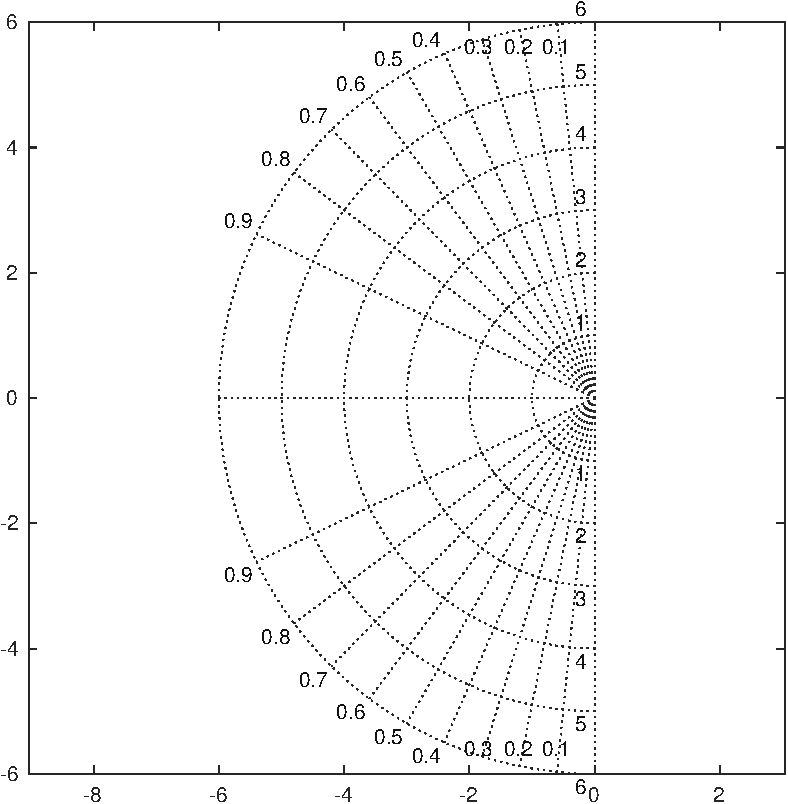
\includegraphics[width=0.41\linewidth]{../../figures/sgrid-crop}
& 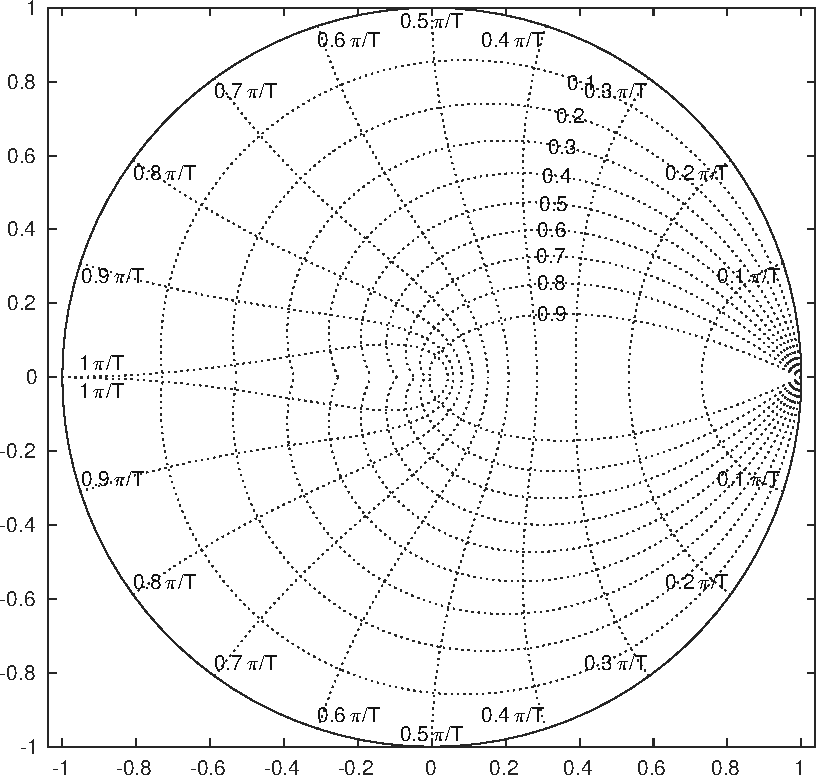
\includegraphics[width=0.43\linewidth]{../../figures/zgrid-crop}\\
s-plane & z-plane
\end{tabular}
\end{center}
\end{frame}
% Emacs 25.3.50.2 (Org mode 8.2.10)
\end{document}